\chapter{Proposta de Solução}

\section{Backlog de Histórias de Usuário ferramenta InvestMVC}

A tabela \ref{backlog} evidencia o Backlog da ferramenta InvestMVC e as respectivas pontuações de cada História de Usuário.

\begin{table}[htp]
\caption{Atividades e objetivos metodologia de pesquisa}
\begin{center}
    \begin{tabular}{ | p{9cm} | p{5cm} |}
    \hline
    \textbf{Histórias de Usuário} & \textbf{Pontuação} \\ \hline

US1 - Agente Correlação Linear & 3\\ \hline
US2 - Agente Fibonacci & 3 \\ \hline
US3 - Agente Mínimos Quadrados & 3\\ \hline
US4 -  Agente Tendência & 2 \\ \hline
US5 - Agente Gestor/Consultor & 2\\ \hline
US6 - Criar conta de usuário & 2\\ \hline
US7 - Acompanhar retorno financeiro & 5\\ \hline
US8 - Criar Experts & 2\\ \hline
US9 - Editar Experts & 2\\ \hline
US10 - Excluir Experts & 2\\ \hline
US11 - Ativar Expert & 1\\ \hline
US12 - Desativar Expert & 2 \\ \hline
US13 - Método Correlação Linear em linguagem C & 2\\ \hline
US14 - Método Fibonacci em linguagem C & 2\\ \hline
US15 - Método Mínimos Quadrados em linguagem C & 2\\ \hline
US16 - Método Correlação Linear em linguagem Haskell & 2\\ \hline
US17 - Método Fibonacci em linguagem Haskell & 2\\ \hline
US18 - Método Mínimos Quadrados em linguagem Haskell & 2\\ \hline
US19 - Inserir na Base de Conhecimento & 2\\ \hline
US20 - Retirar na Base de Conhecimento & 2\\ \hline
US21 - Calcular Critério de Entrada & 3\\ \hline
\textbf{Total de pontos} & 48\\ \hline
\end{tabular}
\end{center}
\label{backlog}
\end{table}

\subsection{Histórias de Usuário}

\subsubsection{Histórias de Usuário Componente MultiAgente}
Nas seções a seguir, são apresentadas as Histórias de Usuário com seus critérios de aceitação referentes ao componente Multiagente.

\textbf{ US1 - Agente Correlação Linear}

Como agente de software, gostaria de usar o método de Correlação de Pearson para verificar sua eficácia no Mercado de Moedas.

Critérios de aceitação US1:

A Correlação de Pearson deve ser maior que 0.8 e o mercado estar subindo para se realizar a venda.

A Correlação de Pearson deve ser maior que 0.8 e o mercado estar caindo para se realizar a compra.

O take profit e o stop loss devem ser os mesmos.

\textbf{US2 - Agente Fibonacci}

Como agente de software, gostaria de usar o método de Fibonacci para verificar sua eficácia no Mercado de Moedas.

Critérios de aceitação US2:

Na situação em que o mercado estiver caindo e a regressão de Fibonacci estiver em 0.62, deve-se apenas vender no mercado com take profit e stop loss em 500 pontos.

Na situação em que o mercado estiver subindo e a regressão de Fibonacci estiver em 0.62, deve-se apenas comprar no mercado com take profit e stop loss em 500 pontos.

\textbf{US3 - Agente Mínimos Quadrados}

Como agente de software, gostaria de usar o método de Mínimos Quadrados para verificar sua eficácia no Mercado de Moedas.

Critérios de aceitação US3:

Não deve existir stop loss ou take profit fixos, pois os mesmos são variáveis de acordo com a estratégia do método de Mínimos Quadrados.

O método deve seguir a tendência do mercado. Se o mercado estiver subindo, deve-se comprar e se estiver caindo, deve-se vender.

\textbf{US4 - Agente Tendência}
Como agente de software, gostaria de verificar a tendência do mercado para estimar um ponto de compra ou venda.

Critérios de aceitação US4:

As cotações obtidas na persistência não podem ser nulas.

A tendência deve ser calculada de acordo com o gráfico escolhido como 1 minuto, 5 minutos e assim por diante.

\textbf{US5 - Agente Gestor/Consultor}

Como agente de software, gostaria de informar ao componente mql uma operação para que seja possível realizar uma compra ou venda.

Critérios de aceitação US5:

Só deve ser informado ao componente mql 1 para compra, -1 para venda ou 0 para fazer nada.

Enquanto o componente mql estiver com uma ordem de compra ou venda aberta, não é necessário informar a operação que deve ser feita ao componente.


\subsubsection{Histórias de Usuário Componente Orientado a Objetos}

Nas seções a seguir, são apresentadas as Histórias de Usuário com seus critérios de aceitação referentes ao componente Orientado a Objetos.

\textbf{US6 - Criar conta de usuário}

Como investidor, gostaria de criar uma conta na ferramenta InvestMVC para que eu possa realizar simulações e/ou investimentos reais.

Critério de aceitação US6:

O usuário deve cadastrar um login que não esteja presente no banco de dados.

O usuário deve cadastrar um senha com 6 digitos.

\textbf{US7 - Acompanhar retorno financeiro}

Como investidor, gostaria de vizualizar o status da minha conta de investidor, para saber o lucro/prejuízo do expert.

Critérios de aceitação US7 :

O retorno é um número real maior que 0.

O tempo de resposta para visualização do saldo deve ser inferior a 2 segundos.

Para acompanhar o retorno financeiro, o usuário deve estar logado na ferramenta InvestMVC.

\textbf{US8 - Criar Experts}

Como investir, gostaria de criar um expert na ferramenta investMVC para que eu possa investir no Mercado de Moedas.

Critérios de aceitação US8 :

Os experts disponíveis devem ser Mínimos Quadrados, Fibonacci e Correlação de Pearson.

Não se pode criar um expert sem ter selecionado ao menos um Método Matemático.

Para criar um expert, o usuário deve estar logado na ferramenta InvestMVC.

\textbf{US9 - Editar Experts}

Como investir, gostaria de editar um expert na ferramenta investMVC para que eu possa investir no Mercado de Moedas.

Critérios de aceitação US9: 

Os experts disponíveis devem ser Mínimos Quadrados, Fibonacci e Correlação de Pearson.

Não se pode editar um expert sem ter selecionado ao menos um Método Matemático para edição.

Para editar um expert, o usuário deve estar logado na ferramenta InvestMVC.


\textbf{US10 - Excluir Experts}

Como investir, gostaria de excluir um expert na ferramenta investMVC para que não mais visualizar o mesmo para investir no Mercado de Moedas.

Critérios de aceitação US10:

Os experts disponíveis devem ser Mínimos Quadrados, Fibonacci e Correlação de Pearson.

Não se pode excluir um expert sem ter selecionado ao menos um Método Matemático para exclusão.

Para excluir um expert, o usuário deve estar logado na ferramenta InvestMVC.


\textbf{US11 - Ativar Expert}

Como investidor, gostaria de ativar um Expert para que o mesmo esteja disponível para operar de forma automatizada.

Critérios de aceitação US11:

Só pode ser ativado um expert que acabou de ser criado ou que está desativado.

Para ativar um expert, o usuário deve estar logado na ferramenta InvestMVC.

\textbf{US12 - Desativar Expert}

Como investidor, gostaria de desativar um Expert para que o mesmo esteja disponível para operar de forma automatizada.

Critérios de aceitação US12:

Só pode ser desativado um expert que esteja ativado.

Para desativar um expert, o usuário deve estar logado na ferramenta InvestMVC.

\subsubsection{Histórias de Usuário Componente Estruturado}
Nas seções a seguir, são apresentadas as Histórias de Usuário com seus critérios de aceitação referentes ao componente Estruturado.

\textbf{US13 - Método Correlação Linear em linguagem C}

Como investidor, gostaria de usar o método de Correlação de Pearson para operar no Mercado de Moedas.

Critérios de aceitação US13:

A Correlação de Pearson deve ser um número real menor que 1 e maior que -1.

Caso, as cotações lidas da persistência sejam nulas, o cálculo é abortado.

\textbf{US14 - Método de Fibonacci em linguagem C}

Como investidor, gostaria de usar o método de Fibonacci para operar no Mercado de Moedas.

Critérios de aceitação US14:

As regressões de Fibonacci devem ser maior que 0 e menor que 1.

Caso, as cotações lidas da persistência sejam nulas, o cálculo é abortado.

\textbf{US15- Método de Mínimos Quadrados em linguagem C}

Como investidor, gostaria de usar o método de Mínimos Quadrados para operar no Mercado de Moedas.

Critérios de aceitação US15:

O coeficiente angular e linear da reta de Mínimos Quadrados são números reais menores que 100.

Caso, as cotações lidas da persistência sejam nulas, o cálculo é abortado.

\subsubsection{Histórias de Usuário Componente Funcional}
Nas seções a seguir, são apresentadas as Histórias de Usuário com seus critérios de aceitação referentes ao componente Funcional.

\textbf{US16- Método Correlação Linear em linguagem Haskell}

Como investidor, gostaria de usar o método de Correlação de Pearson para operar no Mercado de Moedas.

Critérios de aceitação US16:

A Correlação de Pearson deve ser um número real menor que 1 e maior que -1.

Caso, as cotações lidas da persistência sejam nulas, o cálculo é abortado.

\textbf{US17 - Método de Fibonacci em linguagem Haskell}

Como investidor, gostaria de usar o método de Fibonacci para operar no Mercado de Moedas.

Critérios de aceitação US17:

As regressões de Fibonacci devem ser maior que 0 e menor que 1.

Caso, as cotações lidas da persistência sejam nulas, o cálculo é abortado.

\textbf{US18 - Método de Mínimos Quadrados em linguagem Haskell}

Como investidor, gostaria de usar o método de Mínimos Quadrados para operar no Mercado de Moedas.

Critérios de aceitação US18:

O coeficiente angular e linear da reta de Mínimos Quadrados são números reais menores que 100.

Caso, as cotações lidas da persistência sejam nulas, o cálculo é abortado.

\subsubsection{Histórias de Usuário Componente Lógico}

Nas seções a seguir, são apresentadas as Histórias de Usuário com seus critérios de aceitação referentes ao componente Lógico.	

\textbf{US19 - Inserir na Base de Conhecimento}

Como agente de software, gostaria de enviar o retorno do Método Matemático de Correlação de Pearson, Mínimos Quadrados ou Fibonacci para que possa ser inserido na Base de Conhecimento.

Critérios de aceitação US19:

O valor a ser inserido na Base de Conhecimento é um número real.

Não devem ser inseridos valores nulos na Base de Conhecimento.

Caso, seja inserido um valor já existente na Base de Conhecimento, esse valor ganhar um peso a mais na base.

\textbf{US20 - Retirar na Base de Conhecimento}

Como agente de software, gostaria de enviar o retorno do Método Matemático de Correlação de Pearson, Mínimos Quadrados ou Fibonacci para que possa ser retirado na Base de Conhecimento.

Critérios de aceitação US20:

Após o valor ser retirado, deve-se verificar se o mesmo não existe na Base de Conhecimento ou perdeu um peso caso tenha mais de um valor na base.

Deve ser verificado se o valor existe antes do mesmo ser retirado da Base de Conhecimento.

\textbf{US21 - Calcular Critério de Entrada}

Como agente de software, gostaria de solicitar o retorno do Método Matemático de Correlação de Pearson, Mínimos Quadrados ou Fibonacci da Base de Conhecimento para que seja possível operar no Mercado de Moedas.

Critérios de aceitação US21 :

O critério de entrada deve variar de acordo com a estratégia escolhida.

Não devem ser fornecidos critérios de entrada nulos.

\section{Arquitetura Orientada a Componentes}

Arquitetura Orientada a Componentes possui o propósito de dividir para conquistar. Um grande problema é quebrado em partes menores e em seguida se desenvolve soluções mais elaboradas \cite{john}.

Por usar vários paradigmas, a ferramenta InvestMVC terá vários componentes e cada componente terá seu paradigma de programação e responsabilidade bem definida, como mostrado na figura \ref{componente}.

\begin{figure}[htp]
\centering
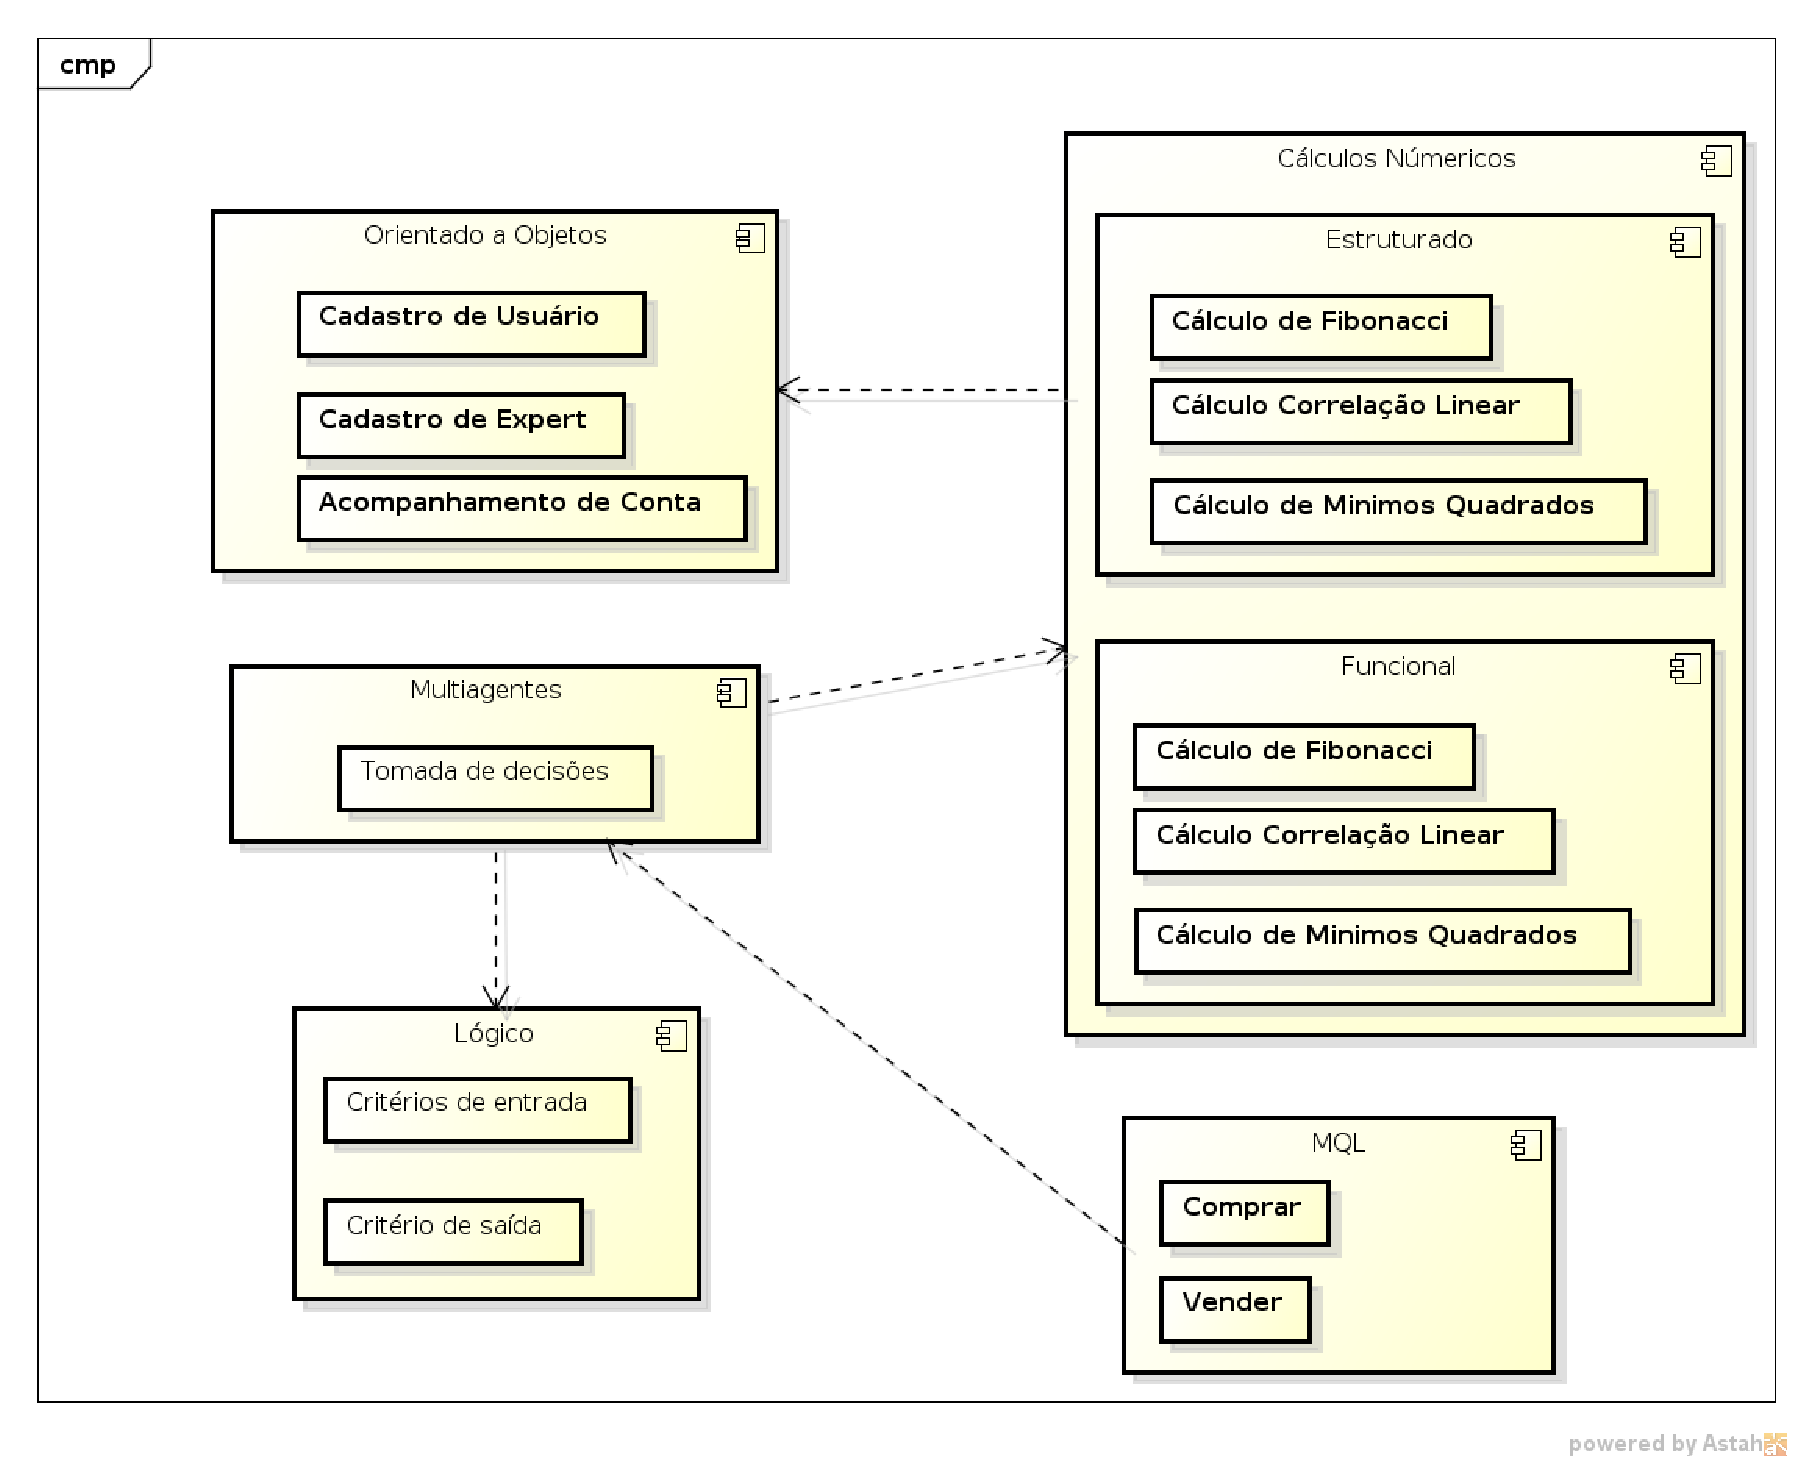
\includegraphics[width=0.9\textwidth]{figuras/componente}
\caption{Diagrama de Sequência InvestMVC}{Fonte:Autores}
\label{componente}
\end{figure}

\subsection{Componente Orientado a Objetos}

Este componente fará a interação com o usuário e será implementado em linguagem Grovvy. A escolha dessa linguagem, se deu porque esta é voltada para aplicações web e juntamente com  o framework grails, fornece a criação de um projeto com uma arquitetura MVC definida, como demonstra a figura \ref{classeOO}.

\begin{figure}[htp]
\centering
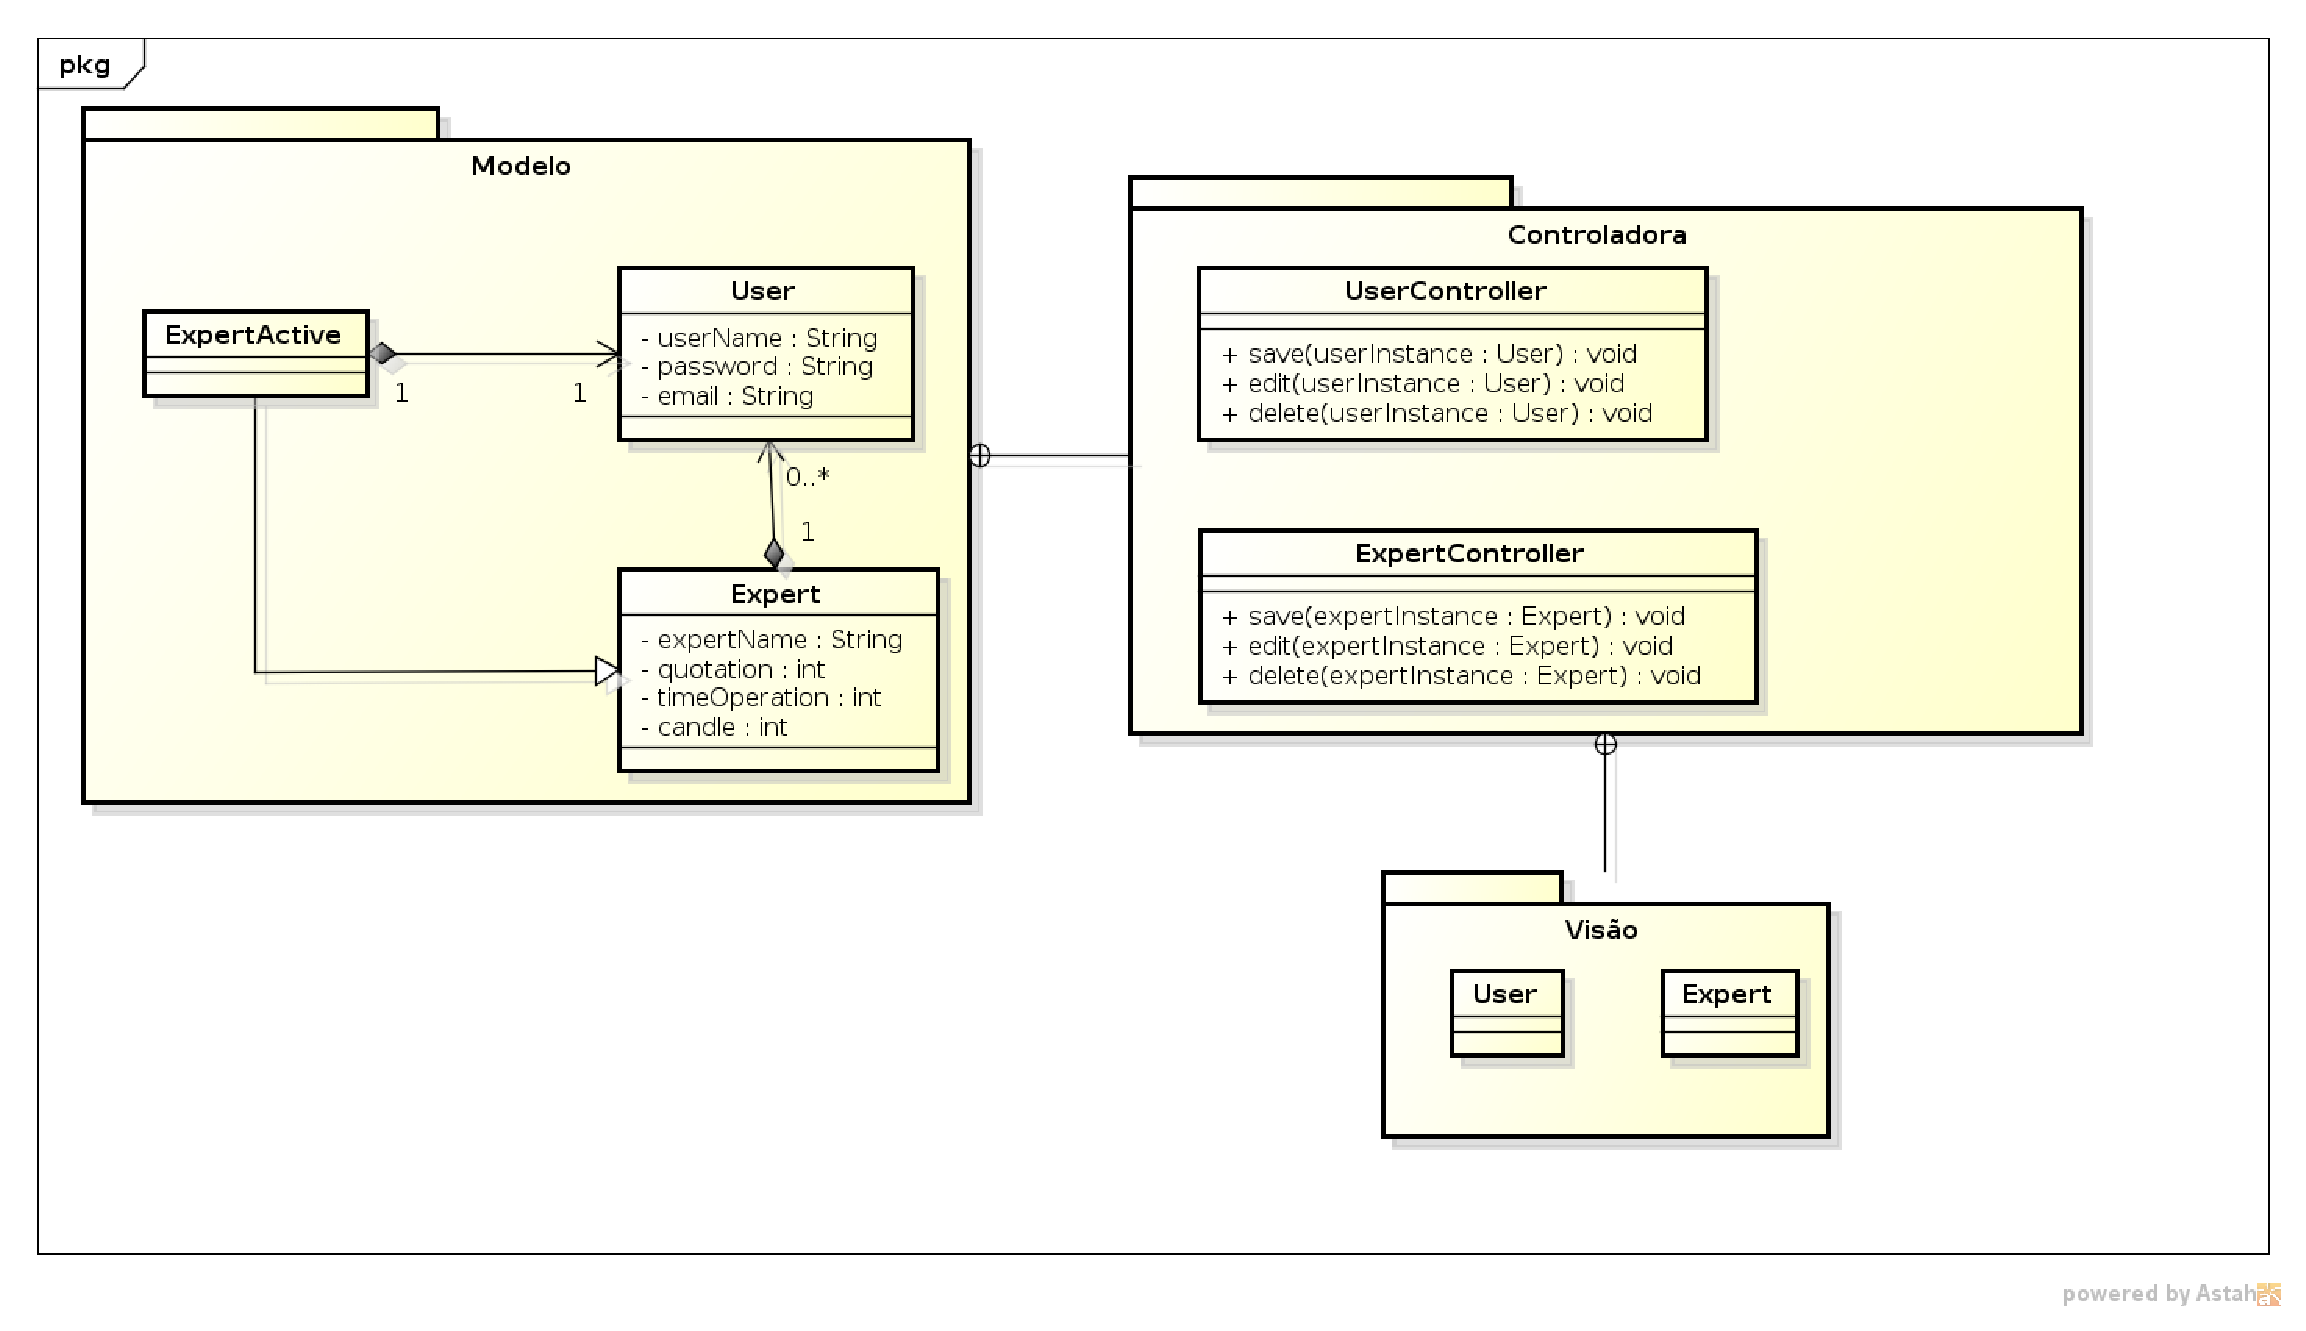
\includegraphics[width=0.9\textwidth]{figuras/classeOO}
\caption{Diagrama de Classe InvestMVC componente Orientado a Objetos}{Fonte: Autores} 
\label{classeOO}
\end{figure}

Segundo \citeonline{lamin} na arquitetura MVC o controle de fluxo de dados dentro deste módulo ocorre da seguinte forma:

\begin{enumerate}
\item O usuário,neste caso o investidor, interage com a Visão;
\item A Controladora manipula o evento da interface do usuário através de uma rotina.
\item A Controladora acessa o Model, atualizando-o baseado na interação do usuário.
\end{enumerate}

Conforme mostra a figura \ref{sequenciaOO}

\begin{figure}[htp]
\centering
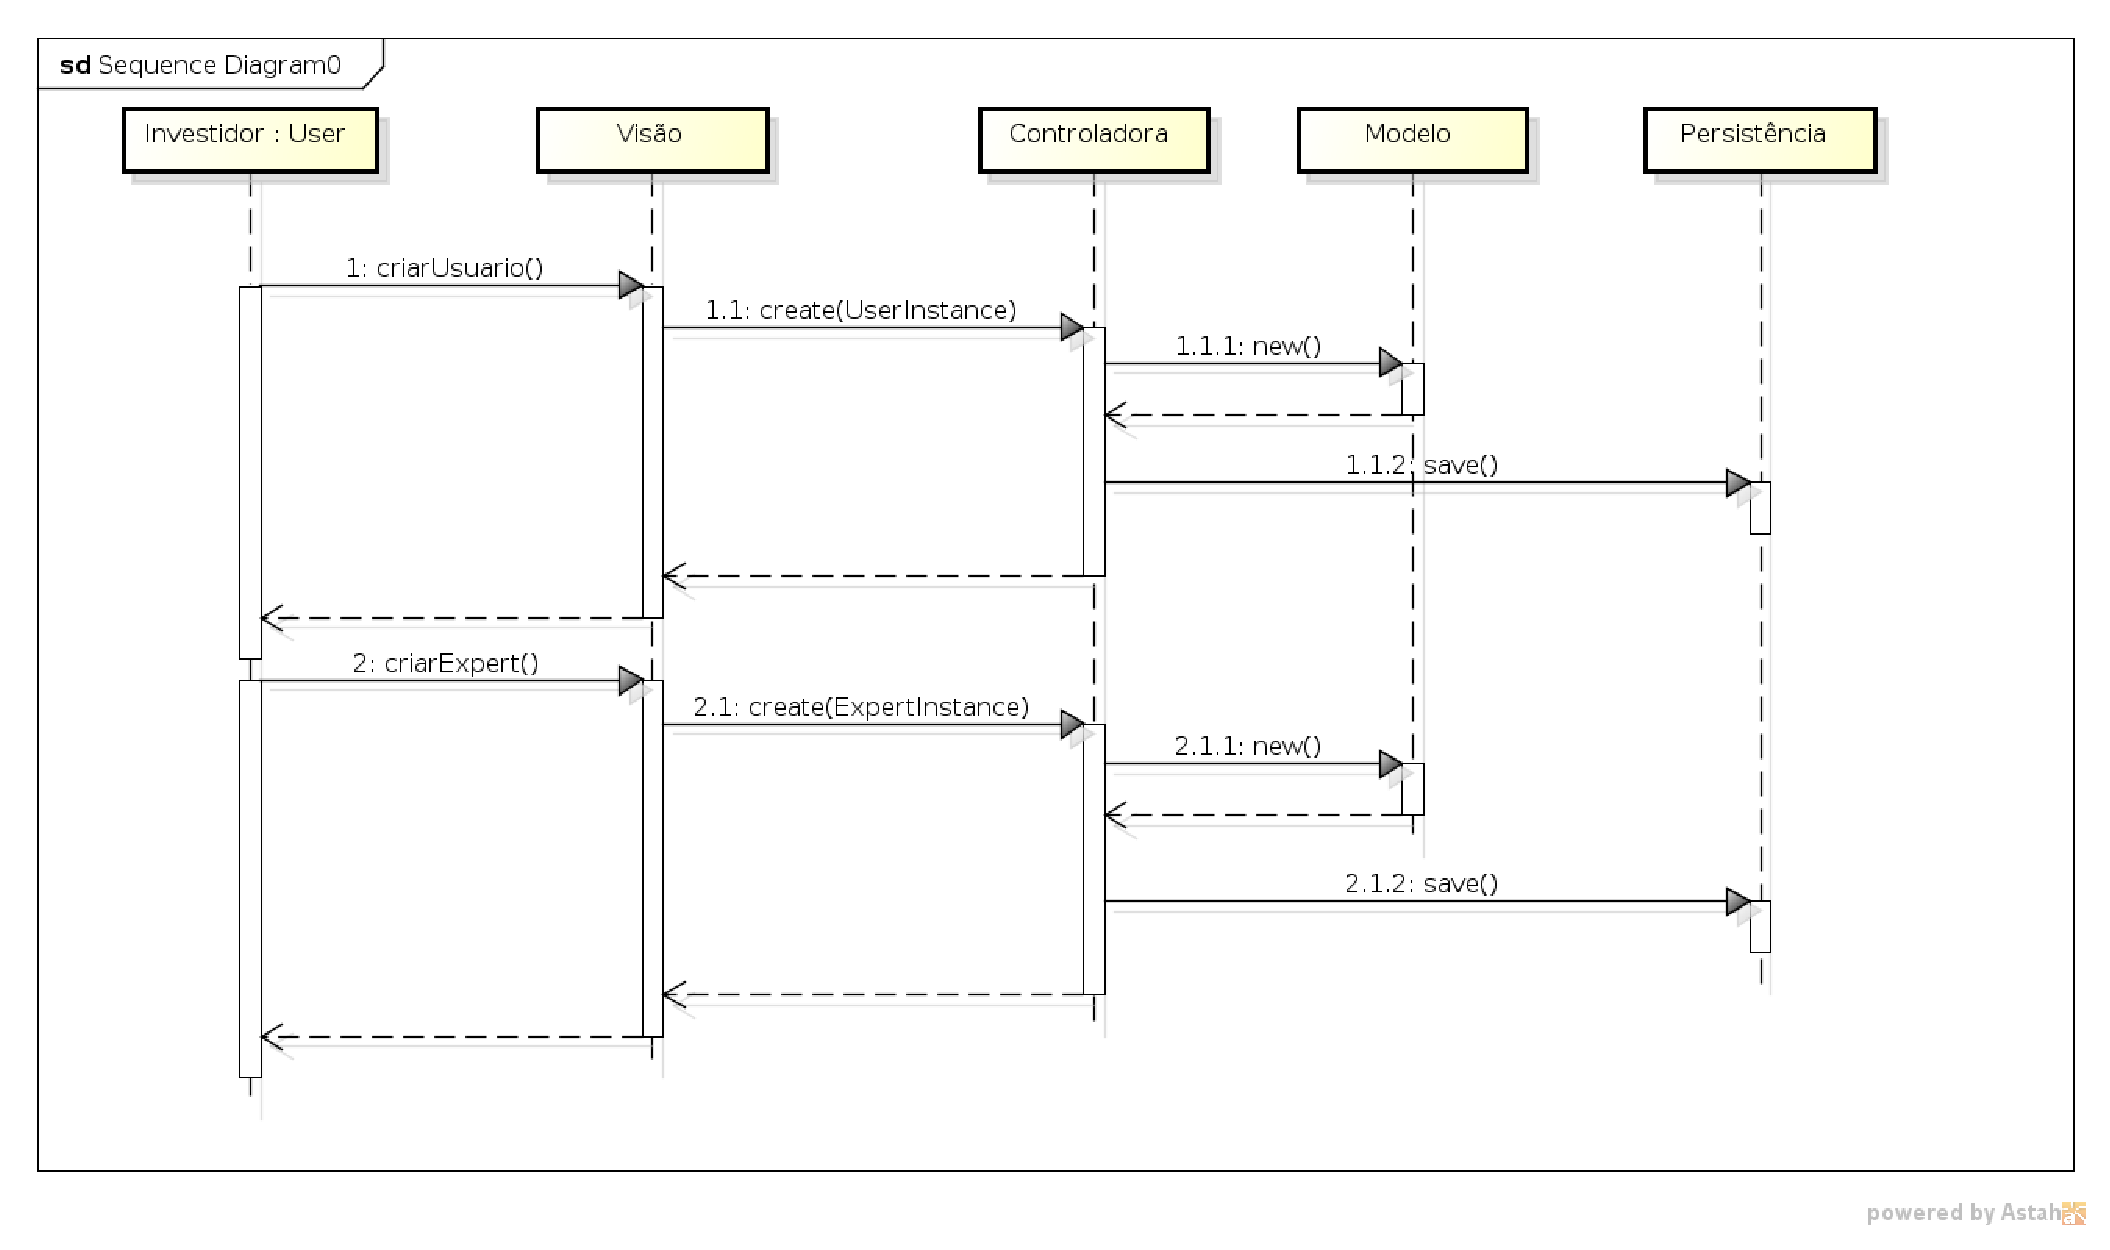
\includegraphics[width=0.9\textwidth]{figuras/sequenciaOO}
\caption{Diagrama de sequência InvestMVC componente Orientado a Objetos}{Fonte: Autores}
\label{sequenciaOO}
\end{figure}

\subsection{Componente Cálculos Numéricos}

O componente Cálculos Numéricos será responsável por calcular os métodos matemáticos presentes na ferramenta InvestMVC. Este módulo é composto por dois outros módulos: módulo Estruturado e módulo Funcional.

O componente Estruturado da ferramenta InvestMVC será programado em linguagem C e o módulo Funcional em linguagem Haskell. Ambos os componentes irão realizar os mesmos cálculos. Isso aumenta a probabilidade de não ocorrer erros nos cálculos dos Métodos Matemáticos. Caso um dos componentes por algum motivo não seja executado no momento correto, a tendência é que o outro módulo realize os cálculos.

\subsubsection{Componente Funcional}
Por ser uma linguagem de programação funcional sua "gramática" está próxima das funções matemáticas, logo a implementação dos métodos algébricos e numéricos se torna muito intuitiva. \cite{hoogle2013}.

O paradigma funcional é declarativo, por limitar o uso de atribuições à variáveis suas funções são mais precisas do que em outros paradigmas \cite{piponi2006}.

Devido aos fatos externalizados, o paradigma funcional, foi eleito para implementar os Métodos Matemáticos de Correlação Linear, Mínimos Quadrados e Fibonacci. Por ser simples,este componente será formado apenas por seus 4 arquivos haskell, cada arquivo realiza o cálculo de um Método Numérico, com execeção do arquivo  Arquivos.hs, que faz a leitura de arquivos.

\begin{figure}[htp]
\centering
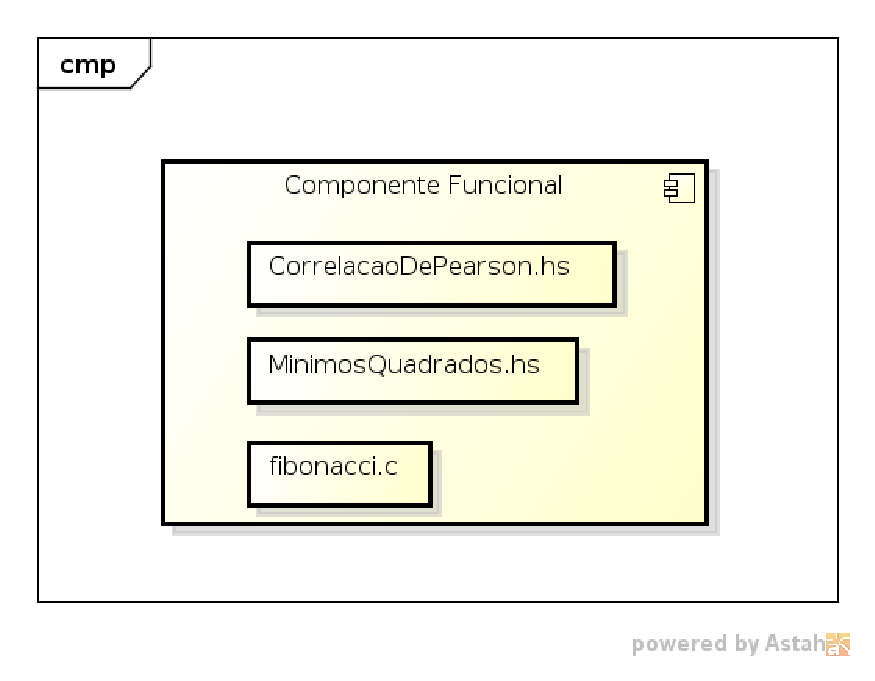
\includegraphics[width=0.5\textwidth]{figuras/componenteFuncional}
\caption{Componente Funcional InvestMVC}{Fonte: Autores} 
\label{componenteFuncional}
\end{figure}

O componente Funcional espera uma socilitação de cálculo do componente Multiagente, logo após a solicitação o componente busca na persistência(um arquivo) as cotações do mercado, com estas cotações o componente é capaz de realizar o cálculo do Método Numérico que é esperado pelo componente Multiagente, como é mostrado na figura \ref{sequenciaFuncional}.

\begin{figure}[htp]
\centering
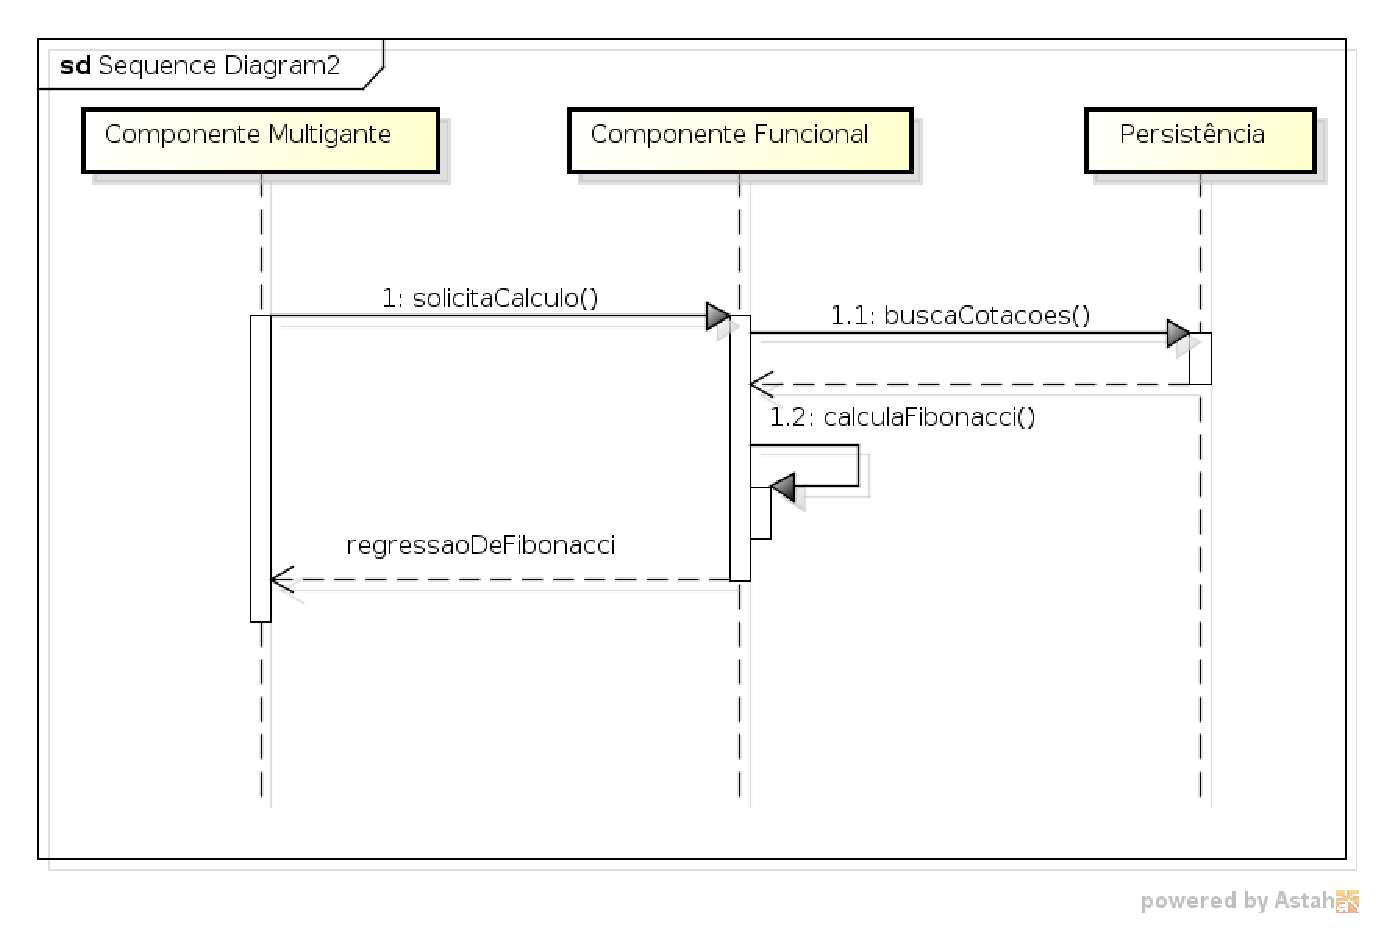
\includegraphics[width=0.9\textwidth]{figuras/sequenciaFuncional}
\caption{Diagrama de Sequência do Componente Funcional InvestMVC}{Fonte: Autores} 
\label{sequenciaFuncional}
\end{figure}

\subsubsection{Componente Estruturado}

A linguagem de programação C é estruturada e possui a vantagem da velocidade de execução do código fonte. Também é uma linguagem bastante utilizada para realizar cálculos numéricos e algébricos \cite{gustavo}. 

Devido aos fatos externalizados, o paradigma estruturado utilizando a linguagem C, também foi eleito para implementar os Métodos Matemáticos de Correlação Linear, Mínimos Quadrados e Fibonacci.

A arquitetura e sequência do fluxo de dados do Componente Estruturado segue a mesma lógica do Componente Funcional, como ilustrado na figura \ref{sequenciaEstruturado}.

\begin{figure}[htp]
\centering
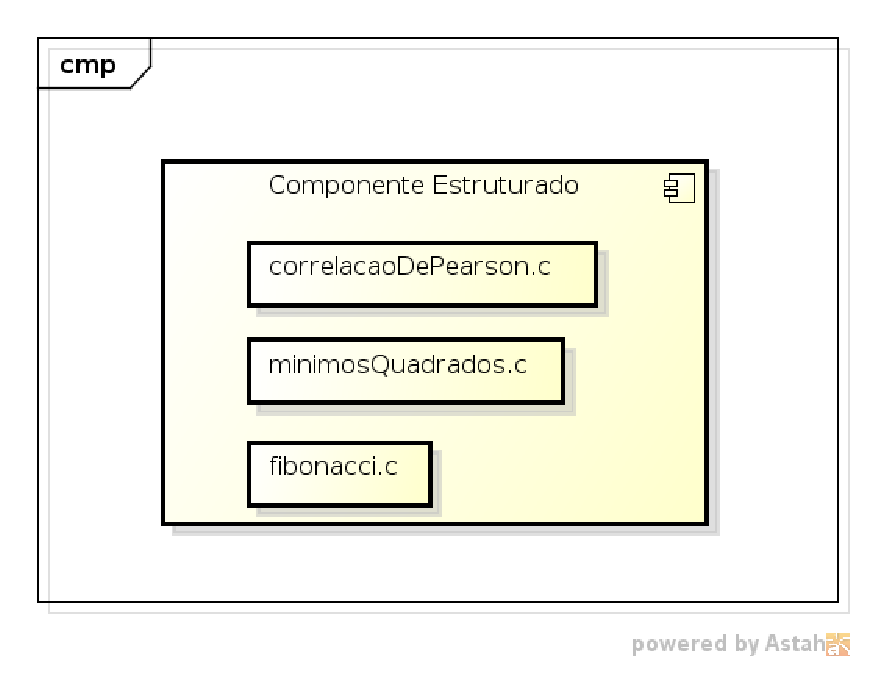
\includegraphics[width=0.5\textwidth]{figuras/componenteEstruturado}
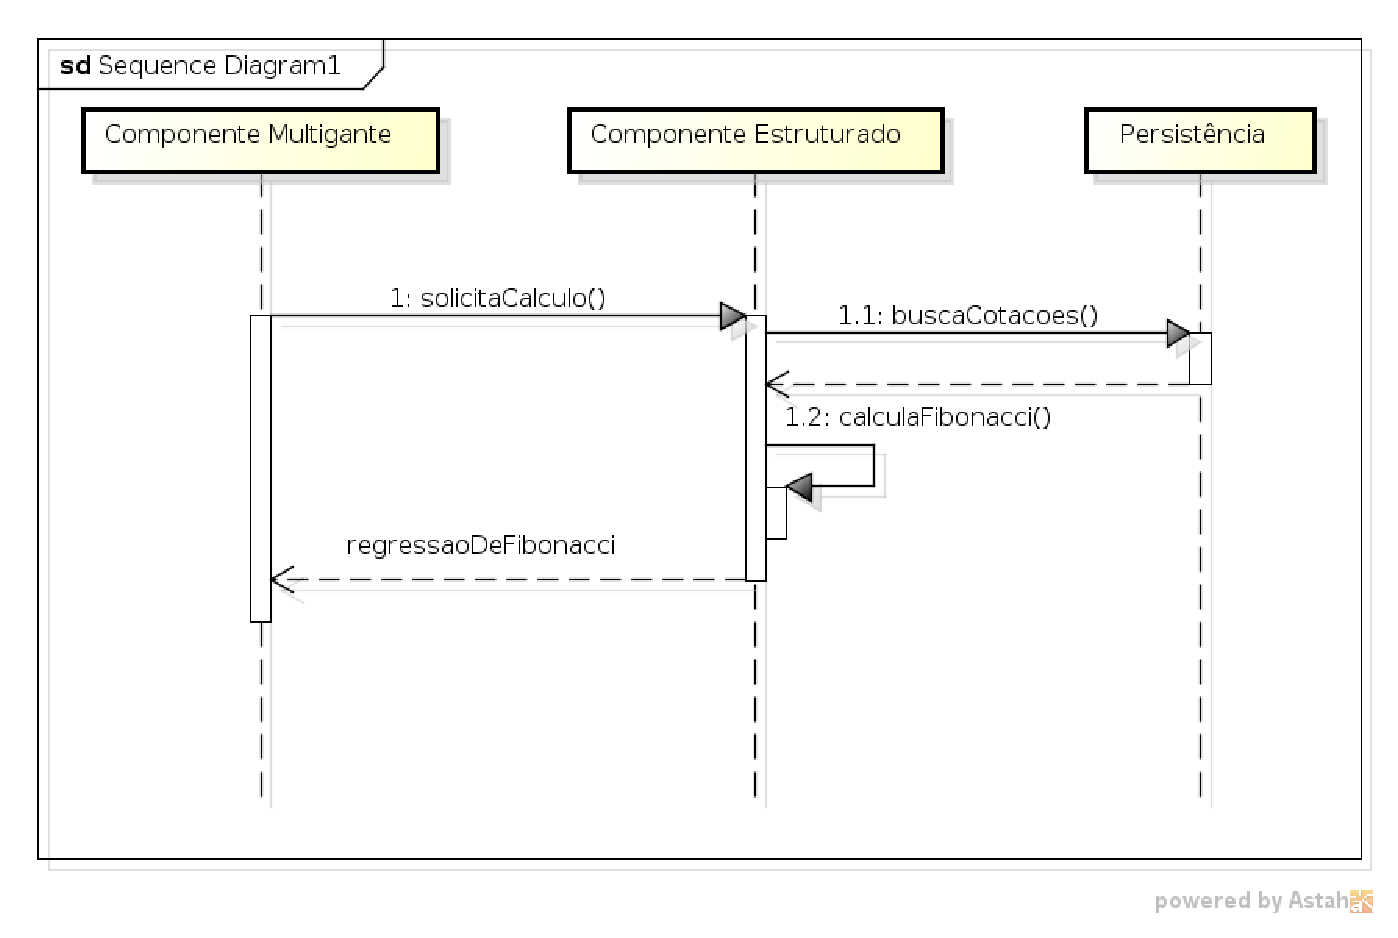
\includegraphics[width=0.5\textwidth]{figuras/sequenciaEstruturado}
\caption{Diagramas de Componentes e de Sequência do Componente Estruturado InvestMVC.}{Fonte: Autores.} 
\label{sequenciaEstruturado}
\end{figure}

\subsection{Componente Multiagentes}

O componente Multiagente será implementado usando o paradigma Multiagente com linguagem Java. 

Agentes de software são entidades autônomas e com capacidades sociais, o uso deste paradigma justifica-se na tomada de decisões \cite{agentBuilderWhy}. 

Os agentes da ferramenta  InvestMVC possuem uma arquitetura reativa, pois suas ações se dão pelas variações que ocorrem nas cotações do Mercado de Moedas.

A arquitetura do Componente Multiagente está modularizado por pacotes: o pacote comportamentos será formado por compormentos que serão usados pelos Agentes de Software, o pacote metodosNumericos será formado por Agentes que acerão o componente Cálculos Numéricos, o pacote investidores será composto por Agentes que vão interagir com o Componente MQL e o pacote execucao iniciará a execução do SMA.

\begin{figure}[htp]
\centering
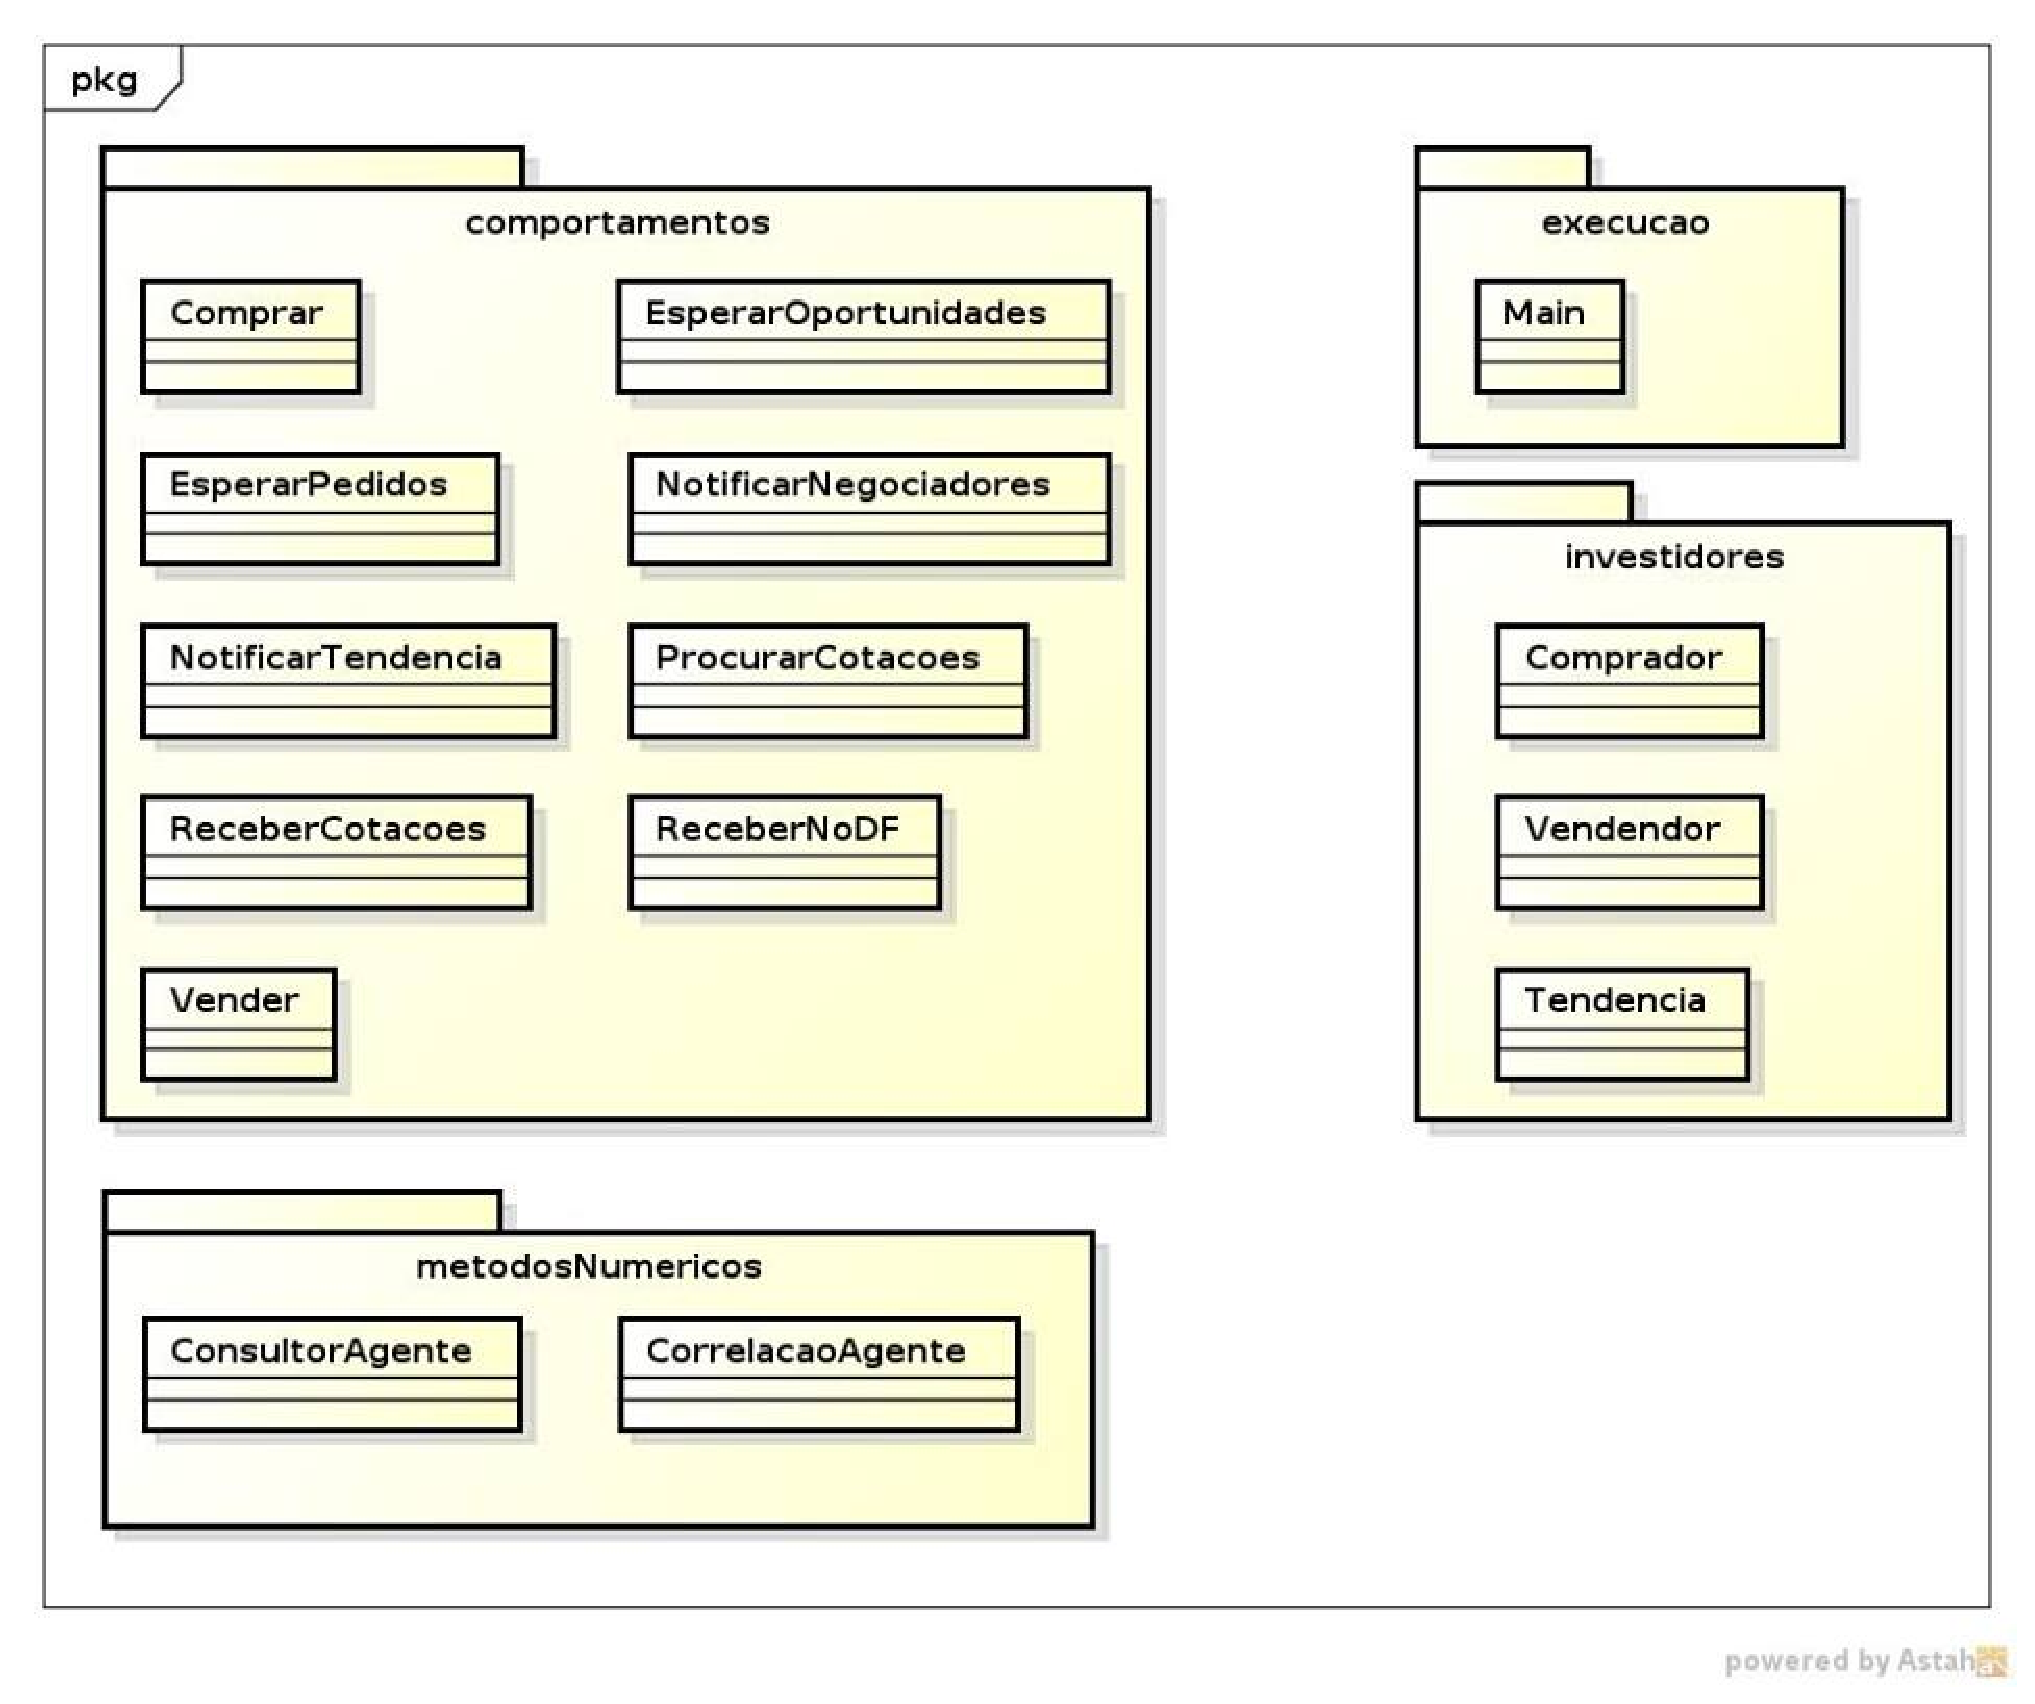
\includegraphics[width=0.9\textwidth]{figuras/diagramaClassesSMA}
\caption{Diagrama de Classe do Componente Multiagente InvestMVC}{Fonte: Autores} 
\label{diagramaClassesSMA}
\end{figure}

\subsection{Componente Lógico}

O componente Lógico será produzido em linguagem Prolog e vai definir uma base de conhecimento que servirá como critério de entrada e saída no Mercado de Moedas.

O paradigma Lógico facilita a representação, inserção e recuperação de conhecimento, por isso é muito usado em aplicações com Inteligência Artificial \cite{almeida2010}.

\subsection{Componente MQL}

O componente MQL será responsável por receber a resposta do módulo Multiagentes para realizar uma compra ou venda. Também será recebido outros atributos relacionados a compra ou venda, como alavancagem, stop loss e take profit.

\subsection{Fluxo de atividades  da ferramenta InvestMVC}

O investidor interage apenas com o componente Orientado a Objetos, criando seu usuário e Experts, no qual serão persistidos. Além disso, o investidor também poderá ativar um Expert.

O componente Multiagentes vai verificar a tendência do Mercado de Moedas, por meio da plataforma MetaTrader. Sendo assim, o componente Multiagentes buscará na persistência o Expert que está ativo. Sabendo qual o Expert que foi ativado, o componente Multiagente faz a requisição de cálculos para os módulos C e Haskell. A partir desse resultado, o componente Multiagente procurará no Módulo Base de Conhecimento, a alavancagem (quanto deve arriscar) e os valores de entrada para o método de Correlação de Pearson, Fibonacci e Mínimos Quadrados. Caso todas as especificações para o módulo Multiagentes sejam obedecidas, ele informa ao componente MQL para realizar uma compra ou venda.

\begin{figure}[htp]
\centering
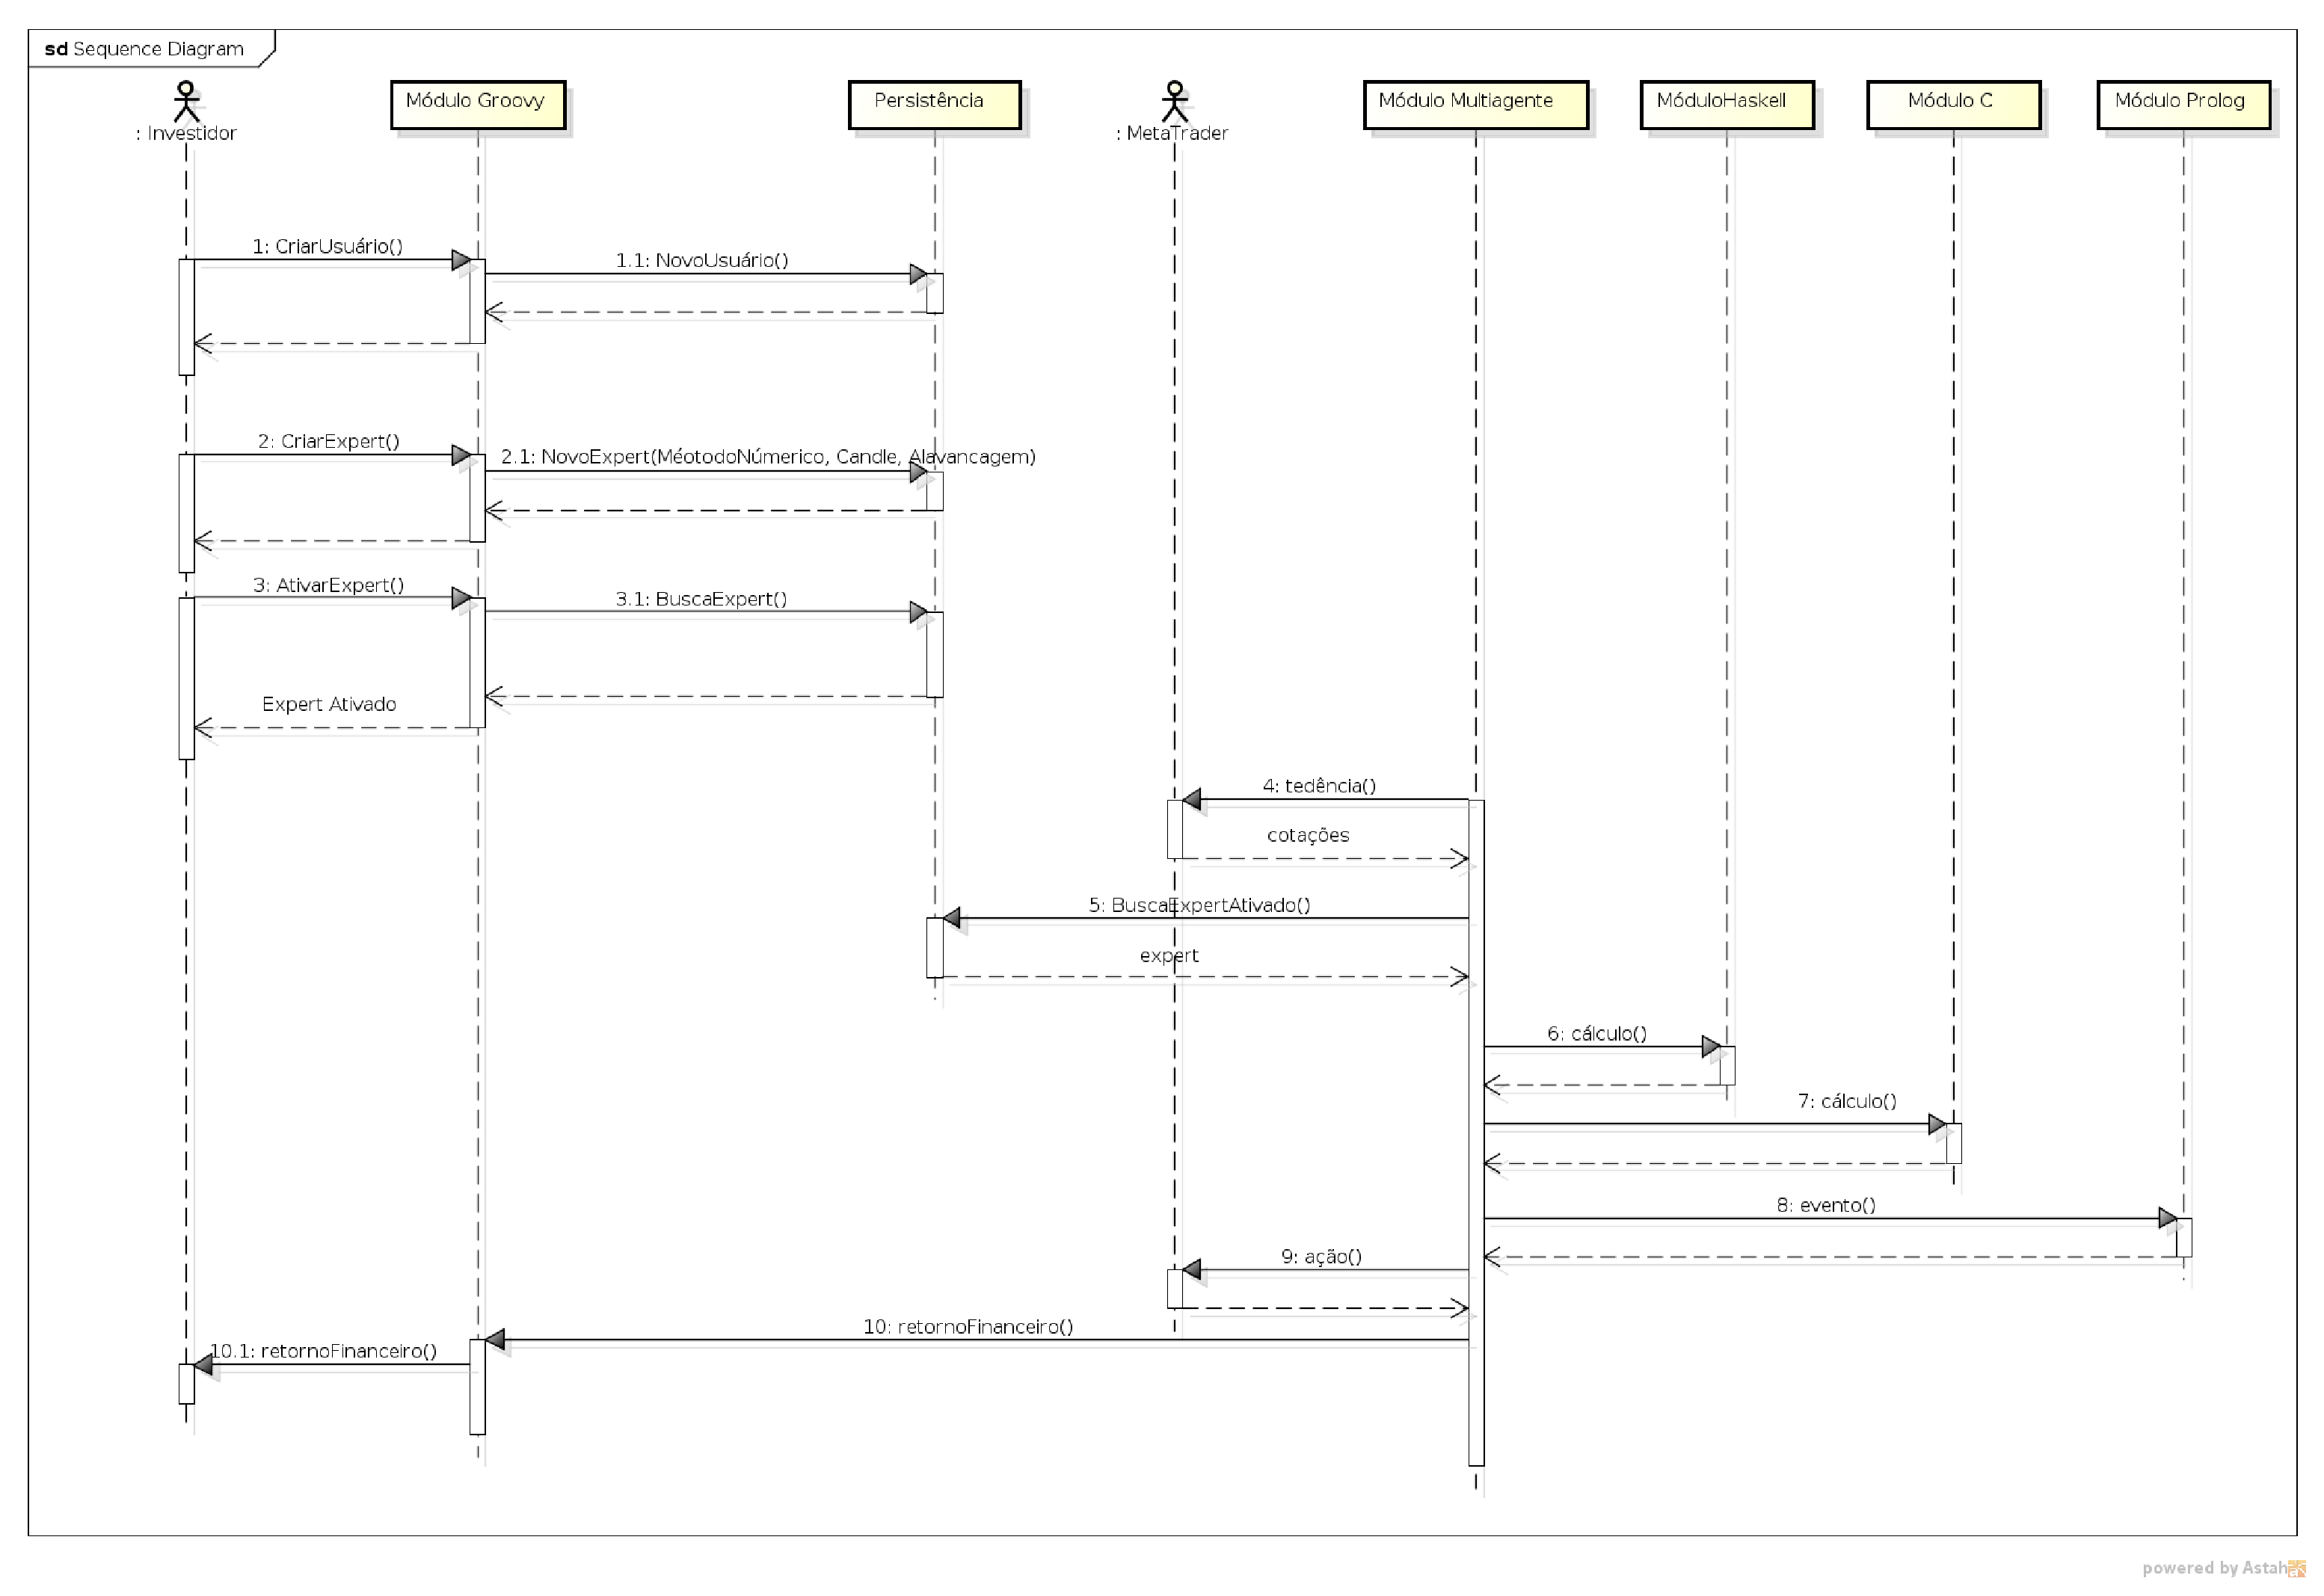
\includegraphics[width=0.9\textwidth]{figuras/sequencia}
\caption{Diagrama de Sequência InvestMVC}{Fonte: Autores} 
\label{sequencia}
\end{figure}
